\documentclass[border=3pt]{standalone}
% Preâmbulo compartilhado pelos diagramas TikZ da aula 11 (Localização por Grade e Monte Carlo)
\usepackage[T1]{fontenc}
\usepackage[utf8]{inputenc}
\usepackage{lmodern}
\usepackage{amsmath}
\usepackage{xcolor}
\usepackage{tikz}
\usetikzlibrary{arrows.meta,angles,quotes,decorations.pathmorphing,calc,
                positioning,shapes.geometric,shapes.misc,backgrounds,fit,
                math}

% Paleta (mesma dos SVGs originais)
\definecolor{dblue}{HTML}{2A5B8C}
\definecolor{dorange}{HTML}{B3541E}
\definecolor{dgreen}{HTML}{4A7C59}
\definecolor{dred}{HTML}{9C4B4B}
\definecolor{dcream}{HTML}{F4F1EA}
\definecolor{dshade}{HTML}{DDD7C9}

% Função gaussiana (não normalizada por padrão de escala visual)
\pgfmathdeclarefunction{gauss}{3}{%
  \pgfmathparse{1/(#3*sqrt(2*pi))*exp(-((#1-#2)^2)/(2*#3^2))}%
}

% Estilos comuns (prefixo d... para não colidir com chaves internas do pgf)
\tikzset{
  >={Stealth[length=2mm]},
  dguide/.style={gray!55, dashed, line width=0.4pt},
  daxis/.style={gray!60, line width=0.7pt, ->},
  dbody/.style={fill=black!3, draw=black!80, line width=1pt},
  dacc/.style={draw=dblue, line width=1pt},
  dlbl/.style={black!55, font=\small},
  dsub/.style={black!45, font=\footnotesize},
  dstate/.style={circle, draw=black!80, fill=dcream, line width=1pt,
                 minimum size=17mm, font=\large, inner sep=1pt},
  dobs/.style={circle, draw=black!80, fill=dshade, line width=1pt,
               minimum size=14mm, font=\large, inner sep=1pt},
  dbox/.style={rounded corners=2pt, draw=black!80, fill=dcream, line width=1pt,
               align=center, inner sep=6pt},
  dop/.style={circle, draw=black!80, fill=white, line width=1pt,
              minimum size=6mm, inner sep=0pt, font=\small},
  dtrans/.style={->, dblue, line width=1pt},
  dmeas/.style={->, dorange, line width=1pt},
  dcurve/.style={line width=1pt, dblue},
  dcurveb/.style={line width=1.4pt, dorange},
}

\begin{document}
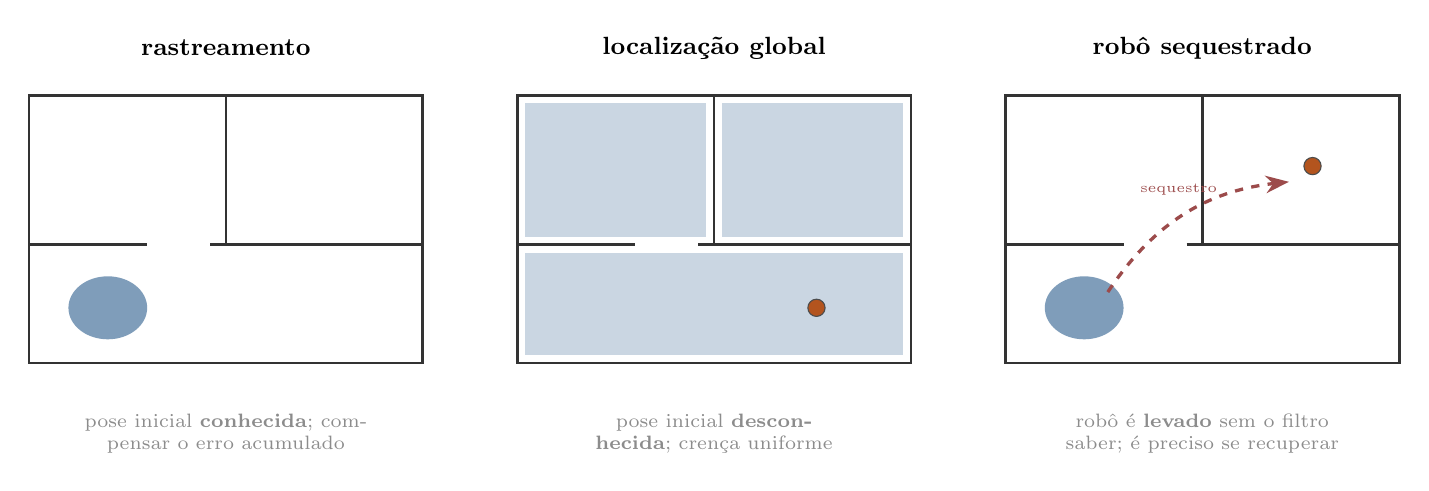
\begin{tikzpicture}[x=1cm,y=1cm,
   rob/.style={circle, fill=dorange, draw=black!70, inner sep=2.2pt},
   bel/.style={fill=dblue!45, draw=dblue, line width=0.6pt}]
  \newcommand{\planta}{\draw[dbody, fill=white, line width=1pt] (0,0) rectangle (5,3.4); \draw[dbody, line width=1pt] (0,1.5) -- (1.5,1.5) (2.3,1.5) -- (5,1.5); \draw[dbody, line width=1pt] (2.5,1.5) -- (2.5,3.4);}
  % tracking
  \begin{scope}
    \planta
    \node[rob] at (1.0,0.7) {}; \fill[dblue!60] (1.0,0.7) ellipse (0.5 and 0.4);
    \node[font=\small\bfseries] at (2.5,4.0) {rastreamento};
    \node[dsub, font=\scriptsize, align=center, text width=4.8cm] at (2.5,-0.9) {pose inicial \textbf{conhecida}; compensar o erro acumulado};
  \end{scope}
  % global
  \begin{scope}[shift={(6.2,0)}]
    \planta
    \fill[dblue!25] (0.1,0.1) rectangle (4.9,1.4); \fill[dblue!25] (0.1,1.6) rectangle (2.4,3.3); \fill[dblue!25] (2.6,1.6) rectangle (4.9,3.3);
    \node[rob] at (3.8,0.7) {};
    \node[font=\small\bfseries] at (2.5,4.0) {localização global};
    \node[dsub, font=\scriptsize, align=center, text width=4.8cm] at (2.5,-0.9) {pose inicial \textbf{desconhecida}; crença uniforme};
  \end{scope}
  % sequestro
  \begin{scope}[shift={(12.4,0)}]
    \planta
    \fill[dblue!60] (1.0,0.7) ellipse (0.5 and 0.4);
    \node[rob] at (3.9,2.5) {};
    \draw[dred, dashed, line width=1.2pt, -{Stealth}] (1.3,0.9) to[bend left=25] (3.6,2.3);
    \node[dred, font=\tiny] at (2.2,2.2) {sequestro};
    \node[font=\small\bfseries] at (2.5,4.0) {robô sequestrado};
    \node[dsub, font=\scriptsize, align=center, text width=4.8cm] at (2.5,-0.9) {robô é \textbf{levado} sem o filtro saber; é preciso se recuperar};
  \end{scope}
\end{tikzpicture}
\end{document}
